%%%%%%%%%%%%%%%%%%%%%%%%%%%%%
%%%%%%%%%%%%%%%%%%%%%%%%%%%%%
% MACRO ATOMS
%%%%%%%%%%%%%%%%%%%%%%%%%%%%%
%%%%%%%%%%%%%%%%%%%%%%%%%%%%%

\section{Macro-atoms}

{\sl The macro-atom scheme was created by Leon Lucy and is outlined in 
his 2002/03 papers. It was implemented in \py\ by Stuart Sim, initially
for the study of recombination lines in YSOs (SDL05).
}

\citet[][hereafter L02, L03]{lucy2002, lucy2003}
has shown that it is possible to calculate the emissivity of a gas in
statistical equilibrium without approximation for problems with large departures
from LTE.
This `macro-atom' scheme allows for all possible transition paths from a given level,
dispensing with the two-level approximation, and
provides a full non-LTE solution
for the level populations based on Monte Carlo estimators. The macro-atom
technique has already been used to model Wolf-Rayet star
winds \citep{sim2004}, AGN disc winds \citep{simlong2008, tatum2012},
supernovae \citep{kromersim2009, kerzendorfsim} and YSOs (SDL05). A full 
description of the approach can be found in L02 and L03. 

The fundamental approach here requires somewhat of a philosophical shift.
Normally MCRT is described in the most intuitive way- that is, we imagine
real photons striking atoms and scattering, or photoionizing 
and depositing energy in a plasma. With Lucy's scheme we should instead 
reimagine the MC quanta as a packets of quantised energy flow, and the scheme as a 
{\em statistical} one. The amount of time a given energy quanta spends in a specific atomic
level or thermal pool is then somewhat analogous to the absolute energy 
contained therein.

Following L02, let us consider an atomic species interacting with a radiation field.
If the quantity $\epsilon_j$ represents the ionization plus excitation energy of 
a level i then the rates at which the level $j$ absorbs and emits radiant energy 
are given by
\begin{equation}
 \dot{A}_{j}^{R} = R_{\ell j} \epsilon_{j \ellp} \;\;\;\;\; {\rm and} \;\;\;
\;\;  \dot{E}_{i}^{R} = R_{j \ellp} \epsilon_{j \ellp} \;\;\; ,
\end{equation}
Where I have adopted Lucy's convention in which the subscript 
$\ellp$ denotes a summation over all lower states ($\ell<j$), and
$\up$ a summation over all upper states ($u>j$).
Similarly, the rates corresponding to {\em kinetic} (collisional)
energy transport can then be written as
\begin{equation}
 \dot{A}_{j}^{C} = C_{\ellp j} \epsilon_{j \ellp} \;\;\;\;\; {\rm and}
\;\;\;
\;\;  \dot{E}_{j}^{C} = C_{j \ellp} \epsilon_{j \ellp} \;\;\; ,
\end{equation}
Let us define ${\cal R}$ as a total rate, such that
${\cal R}_{\ellp j}  = R_{\ellp j} + C_{\ellp j}$.
If we now impose statistical equilibrium
%
\begin{equation}
 ({\cal R}_{\ellp j}-{\cal R}_{j \ellp})+({\cal R}_{\up j}-{\cal R}_{j\up})=0 \;\;\;.
\end{equation}
we can then obtain 
\begin{eqnarray}
 \dot{E}_{j}^{R}+\dot{E}_{j}^{C}+{\cal R}_{j\up}\epsilon_{j}+
 {\cal R}_{j \ell}\epsilon_{\ellp}  \nonumber \\  
 = \dot{A}_{j}^{R}+\dot{A}_{j}^{C}+{\cal R}_{\up j} \epsilon_{j}
 +{\cal R}_{\ellp j} \epsilon_{\ellp}           .  
 \label{eq:matom_SE}     
\end{eqnarray}
This equation is the starting point for the macro-atom scheme. It shows 
that, when assuming radiative equilibrium, the energy flows through
a system depend only on the transition probabilities and atomic physics
associated with the levels the energy flow interacts with.
By quantising this energy flow into radiant ($r$-) and kinetic ($k$-) packets, 
we can simulate the energy transport through
a plasma discretised into volume elements (``macro-atoms''),
whose associated transition probabilities govern the interaction 
of radiant and kinetic energy with the ionization and excitation energy associated 
with the ions of the plasma.

Although equation~\ref{eq:matom_SE} assumes strict radiative equilbrium,
it is trivial to adjust it to include non-radiative source and sink terms. 
For example, in an expanding parcel of plasma, adiabatic cooling may be 
included with a simple modification to the RHS of equation~\ref{eq:matom_SE}.


%%%%%%%%%%%%%%%%%%%%%%%%%%%%%
% PROBS
%%%%%%%%%%%%%%%%%%%%%%%%%%%%%

\subsection{Transition Probabilities}

Having interpreted equation~\ref{eq:matom_SE} in a {\em stochastic} way,
I can now construct a Monte Carlo scheme, following L02.
A macro-atom in state $j$ always has a finite probability of deactivating
radiatively or collisionally:
\begin{equation}
p_{j}^{R} = \dot{E}_{j}^{R} / D_j \;\;\;\;\; {\rm and} \;\;\;
\;\; p_{j}^{C} = \dot{E}_{j}^{C} / D_j,
\label{eq:deactivate}
\end{equation}
where I have defined
\begin{equation}
D_j =  \dot{E}_{j}^{R}+\dot{E}_{j}^{C}+{\cal R}_{j\up}\epsilon_{j}+
 {\cal R}_{j \ellp}\epsilon_{\ellp} = ({\cal R}_{j\ellp} + {\cal R}_{j\up}) \epsilon_{j}.
\end{equation}
The corresponding jumping probabilities, which describe the probability
that the macro-atom transitions to a different state while remaining active, 
are given by
\begin{equation}
p_{j\up} = {\cal R}_{ju} \epsilon_{j} / D_j \;\;\;\;\; {\rm and} \;\;\;
\;\; p_{j\ellp} = {\cal R}_{j\ellp} \epsilon_{\ellp} / D_j.
\end{equation}
Note that the jumping probability is always proportional to the energy
of the lower level, whereas the emission probability is proportional
to the energy {\em difference} between the levels, as 
$\dot{E}_{j}^{R} = R_{j\ellp} (\epsilon_j - \epsilon_\ellp)$. We can also
trivially show that the probabilities are correctly normalised, as
\begin{align}
p_{j}^{R} + p_{j}^{C} + p_{j\ellp} + p_{j\up} &=
(1/D_j) ( {\cal R}_{j\up} \epsilon_{j} + {\cal R}_{j\ellp} \epsilon_{\ellp} +
\dot{E}_{j}^{R} + \dot{E}_{j}^{C}) \\
&= 1. \nonumber
\end{align}

With these transition
probabilities identified, a Monte Carlo calculation can proceed by formulating
the normal statistical equilibrium rate equations that will depend on
the ambient conditions of the plasma. The effect of these ambient conditions
is expressed through the use of Monte Carlo estimators.




%%%%%%%%%%%%%%%%%%%%%%%%%%%%%
% RATES
%%%%%%%%%%%%%%%%%%%%%%%%%%%%%
\subsection{Rate equations}
\label{sec:rate_eq}
The macroscopic transition probabilities above depend on the traditional
rate equations formulated according to statistical equilibrium. 
In the framework of the Sobolev escape probability formalism 
(see section~\ref{sec:sobolev}), 
the bound-bound excitation rate, ${\cal R}_{ju}$, in an ion is given by 
\begin{equation}
{\cal R}_{ju} = B_{ju} n_j J_{est} + q_{ju} n_j n_e,
\label{eq:rad_rate}
\end{equation}
where $u$ is now a specific upper level and $q_{ju}$ is the collisional
rate coefficient (see section~\ref{sec:coll}).
$J_{est}$ is the Monte Carlo estimator for the mean intensity 
impinging on the Sobolev region, weighted by an angle-dependent escape probability, 
given by \citep{sim2004}
\begin{equation}
J_{est} = \frac{c}{4 \pi \nu_{uj} V} \sum_{i}^{\mathrm{photons}} w_i \frac{1 - e^{-\tau_{s,i}}}{\tau_{s,i}} \frac{1}{(dv/ds)_i}.
\end{equation}
Here $w_i$ is the photon weight (in luminosity units), $\nu_{uj}$
is the line frequency, $dv/ds$ is the velocity gradient and
$\tau_s$ is the Sobolev optical depth.
The sum is over all photons that come into resonance with the line,
and thus represents an integral over solid angle.
This is essentially the MC estimator form of $\beta_{uj}\bar{J}_{uj}$, and differs
from the estimator in equation~(20) of L02 as 
there is no assumption of homologous flow or symmetric escape probabilities.
The corresponding de-excitation rate is then 
\begin{equation}
{\cal R}_{uj} = \beta_{ju} A_{uj} n_u + B_{uj} n_u J_{est} +
q_{uj} n_u n_e.
\label{eq:nlte_rul}
\end{equation}
In practice, the stimulated emission term is included as a negative contribution
to the radiative excitation rate, requiring no population inversions 
(see section~\ref{sec:numerical_matom}).
The photoionization and collisional ionization rates
between a lower level, $l$, and the continuum level $\kappa$ 
(or, in the case of ions with more than one bound electron, 
the ground state of the upper ion),
$\kappa$, are
\begin{equation}
{\cal R}_{j \kappa}= n_j (\gamma_{j\kappa} - \alpha^{st}_{\kappa j})  + q_{j \kappa} n_j n_e.
\end{equation}
Here, $q_{j \kappa}$ is the collisional ionization rate coefficient, 
$\gamma_{j \kappa}$ is the photoionization rate
from $j \rightarrow \kappa$ and $\alpha^{st}_{\kappa j}$ is the stimulated recombination
coefficient. This is included as a negative photoionization term rather 
than a positive recombination term as in L03, which requires that there are
no population inversions (see section~\ref{sec:numerical_matom}). 
The corresponding recombination rate is given by 
\begin{equation}
{\cal R}_{\kappa j} = \alpha_{\kappa j} n_{\kappa} n_e + q_{\kappa j}
n_\kappa n_e, \\
\end{equation}
where $\alpha_{\kappa l}$ is the radiative recombination coefficient
to level $l$, and is given by 
\begin{equation}
\alpha_{\kappa j} = 4\pi \Phi^*_{j\kappa} \int^\infty_{\nu_0} 
\frac{\sigma_{j\kappa} (\nu)}{h \nu} \frac{2 h \nu^3}{c^2} 
\exp \left( \frac{- h \nu}{k T_e} \right) d\nu.
\label{eq:alpha_sp}
\end{equation}
This treatment means that radiative and collisional
rates to and from all levels can be considered when calculating the
ionization state, level populations and transition probabilities, 
although ionization directly to excited levels of the upper ion is 
neglected. 

\subsubsection{Collision Strengths}
\label{sec:coll}

The bound-bound collisional rate coefficient $q_{lu}$ is calculated from the
\cite{vanregemorter} approximation, given by
\begin{equation}
q_{ju} = 2.388 \times 10^{-6}~\lambda_{uj}^3~A_{uj}~g_u~\bar{g},
\label{eq:vanregemorter}
\end{equation}
where $\lambda_{uj}$ is the wavelength of the transition and $\bar{g}$ is 
an effective gaunt factor of order unity.
The inverse rate can just be calculated by considering detailed balance, 
such that
\begin{equation}
q_{uj} = q_{ju} \frac{g_u}{g_j} \exp \left( \frac{h \nu_{uj}}{k T_e} \right)
\label{eq:vanregemorter2}
\end{equation}
Using equation~\ref{eq:vanregemorter} means that collisions between radiatively
forbidden transitions are not taken into account when one 
splits levels into $l$- and $s$-subshells, as well
as principal quantum number, $n$ (as done with He~\textsc{i}; 
see chapter 4). Although this approximation is, in general, 
a poor one, the effect is second order in the physical 
regime where recombination lines are formed in our models. 
This is because bound-free processes are dominant in determining 
level populations and emissivities. I have verified that this 
is indeed the case in the He~\textsc{i} emission regions in the models
presented here.

The bound-free collision strengths are calculated using equation~(5.79) of
\cite{mihalas}. The collisional ionization rate coefficient is
\begin{equation}
q_{j\kappa} = 1.55 \times 10^{-13} n_e~\bar{g}_{i}~\sigma_{j\kappa} (\nu_{\kappa j})~
\frac{h \nu_{\kappa j}}{k T_e^{3/2}}
\exp \left( \frac{- h \nu_{\kappa j}}{k T_e} \right),
\label{eq:qioniz}
\end{equation}
where $\sigma_{j\kappa} (\nu_{\kappa j})$ is the photoionization cross-section 
at the threshold energy.
$\bar{g}_{i}$ is an effective gaunt factor for ion $i$ and is approximately
equal to $0.1,0.2,0.3$ for $Z=1,2$ and $>2$ respectively,
where $Z$ is the atomic number. Note that the use of this estimator
implies a $\nu^{-3}$ shape to the photoionization cross-section,
which is only strictly true for for hydrogenic ions.
The collisional (three-body) recombination rate is found using the Saha equation
and given by
\begin{equation}
q_{\kappa j} = q_{j\kappa} \left( \frac{n_j}{n_e n_\kappa} \right)^*_{T_e}.
\label{eq:qrecomb}
\end{equation}
For numerical reasons, the above two expressions are combined in \py\ where 
possible, to avoid multiplying two exponentials together.





%%%%%%%%%%%%%%%%%%%%%%%%%%%%%
%ESTIMATORS
%%%%%%%%%%%%%%%%%%%%%%%%%%%%%
\subsection{Macro-atom estimators}
\label{sec:estimators}
To be able to solve the above rate equations and compute the transition 
probabilities, it is necessary to construct estimators for the various properties
of the radiation field that appear in said equations. This is done
by converting integrals over the radiation field into summations over 
$r$-packets passing through a cell. This represents the stochastic nature of
a MC simulation, and is by no means unique to the macro-atom formalism.
The first step is to apply the energy-density argument of \cite{lucy1999radeq},
which gives, for a time-independent code
\begin{equation}
J_\nu~d\nu = \frac{1}{4\pi}\frac{1}{V} \sum_{d\nu} w_i \Delta s,
\end{equation}
where the summation is over all photons between $(\nu, \nu+d\nu)$. This allows
the formulation of estimators in a MC sense, rather than in integral form. 

\subsubsection{Bound-free estimators}
The estimator for the photoionization rate is 
\begin{equation}
\gamma_{j\kappa} = \frac{1}{V} \sum_i^{\mathrm{photons}} 
\frac{w_i~\sigma_{j\kappa}({\nu})}{h \nu}~\Delta s
\end{equation}
and for the stimulated recombination rate is
\begin{equation}
\alpha_{\kappa j}^{st} =\left( \frac{n_j}{n_e n_\kappa} \right)^*_{T_e}
\frac{1}{V} \sum_i^{\mathrm{photons}} 
\frac{w_i~\sigma_{j\kappa}({\nu})}{h \nu}
~\exp(-h\nu/kT_e)~\Delta s,
\end{equation}
where $\sigma_{l\kappa} (\nu)$ is the photoionization cross-section for this transition.
We also need to define modified rate coefficients which 
are the rates at which bound-free transitions add energy to and remove energy from 
the radiation field. These are required for photoionization, 
spontaneous recombination and stimulated recombination, and are given by

\begin{equation}
\gamma^E_{j\kappa} = \frac{1}{V} \sum_i^{\mathrm{photons}} 
\frac{w_i~\sigma_{j\kappa}{\kappa j}}{h \nu_{\kappa j}}~\Delta s, 
\end{equation}

\begin{equation}
\alpha^E_{\kappa j} = 4\pi \left( \frac{n_j}{n_e n_\kappa} \right)^*_{T_e}
 \int^\infty_{\nu_{\kappa j}} 
\frac{\sigma_{j \kappa}(\nu)}{h \nu_{\kappa j}} \frac{2 h \nu^3}{c^2} 
\exp \left( \frac{- h \nu}{k T_e} \right) d\nu,
\end{equation}

\begin{equation}
\alpha_{\kappa j}^{st,E} = \left( \frac{n_j}{n_e n_\kappa} \right)^*_{T_e}
\frac{1}{V} \sum_i^{\mathrm{photons}}
\frac{w_i~\sigma_{j\kappa}({\nu})}{h \nu_{\kappa j}}
~\exp(-h\nu/kT_e)~\Delta s.
\end{equation}
The rate at which recombinations convert
thermal {\em and} ionization energy into radiant energy is then
$\alpha^E h\nu_{\kappa j} n_\kappa n_e$, where $h \nu_{\kappa j}$ is the potential of the 
bound-free transition, or the energy difference between continuum $\kappa$ and 
the level $j$ the electron is recombining too. 
The amount of this energy which is removed from the thermal pool
therefore needs a quantity $\alpha_{\kappa j} h\nu_{\kappa j} n_\kappa n_e$ subtracted from it,
giving the bound-free cooling estimator
\begin{equation}
\cc_{bf} = \sum_{j\kappa}^{\mathrm{bfjumps}} 
\left[ (\alpha^E_{\kappa j} + \alpha^{st,E}_{\kappa j} - \alpha_{\kappa j} - \alpha^{st}_{\kappa j}) 
n_{\kappa} + 
q_{j\kappa} n_j \right]
n_e h\nu_{\kappa j} V,
\end{equation}
where the sum is over all the macro-atom bound-free transitions ($j\rightarrow\kappa$) 
in the simulation, set by
the number of photoionization cross-sections. 
For bound-free heating, we write a similar expression. The rate of at which
a level $l$ absorbs energy by bound-free 
transitions is given by $\gamma^E_{j\kappa} h\nu_{\kappa j} n_\kappa n_e$,
but the amount $\gamma_{j\kappa} h \nu_{\kappa j} n_l$ goes into ionization energy, giving 
\begin{equation}
\hh_{bf} = \sum_{j\kappa}^{\mathrm{bfjumps}} \left[ (\gamma^E_{\kappa j} - \gamma_{\kappa j}) n_j + n_\kappa n_e^2 q_{\kappa j} \right] h \nu_{\kappa j} V
\end{equation}
as the rate at which radiant energy heats the plasma via bound-free transitions.

\subsubsection{Bound-bound estimators}
The heating and cooling rates for macro-atom bound-bound transitions are the rates of
collisional excitations and de-excitations
- i.e. the rate at which thermal energy is converted into
bound-bound excitation energy and vice versa.
These heating and cooling rate estimators are:

\begin{equation}
\hh_{bb} = \sum_{ju}^{\mathrm{lines}} q_{uj} n_u n_e h \nu_{uj} V,
\end{equation}


\begin{equation}
\cc_{bb} = \sum_{ju}^{\mathrm{lines}} q_{ju} n_j n_e h \nu_{uj} V.
\end{equation}

\subsubsection{Other heating and cooling estimators}
Although I have now defined the estimators required to calculate the 
transition probabilities, level populations, heating rates and cooling rates in macro-atoms, 
there are still a number of heating and cooling mechanisms that do not involve macro-atoms. 

The free-free cooling estimator is calculated from the emission coefficient
in equation~\ref{eq:jff} 
\begin{equation}
\cc_{ff} = V \sum_i^{\mathrm{ions}} \int \frac{j_{ff,i}(\nu)}{4\pi} d\nu,
\end{equation}
where the integral is over all frequencies included in the simulation,
and the sum is also over all ions included in the simulation.
The corresponding heating rate is then
\begin{equation}
\hh_{ff} = \sum_i^{\mathrm{photons}} w_i \kappa_{ff} \Delta s.
\end{equation}
Compton heating and cooling is included in the thermal balance and as
$(r\rightarrow k)$ and $(k\rightarrow r)$ transitions:
\begin{equation}
\cc_{\mathrm{comp}} = 16 \pi \sigma_T V J \frac{k T_e}{m_e c^2},
\end{equation}
\begin{equation}
\hh_{\mathrm{comp}} = n_e \sum_i^{\mathrm{photons}} \frac{h\nu}{m_e c^2} w_i \kappa_{C}\Delta s,
\end{equation}
where the estimator for the frequency-integrated mean intensity is
\begin{equation}
J = \frac{1}{4\pi V} \sum_i^{\mathrm{photons}} w_i \Delta s.
\label{eq:j}
\end{equation}
Induced Compton heating is then given by \citep{cloudy2013}
\begin{equation}
\hh_{\mathrm{ind~comp}} = n_e \sum_i^{\mathrm{photons}} \frac{J_\nu c^2}{h \nu^3} \frac{h\nu}{m_e c^2} 
w_i \kappa_{C} \Delta s,
\end{equation}
where the first $J_\nu c^2/h \nu^3$ term represents the
photon occupation number, and $J_\nu$ is either 
calculated from the spectral model
described in section~\ref{sec:simple_ionization} or a dilute blackbody.
The adiabatic cooling rate is derived from $PdV$ work and is given by
\begin{equation}
\cc_{a} = k T_e V (\nabla \cdot v) \left(n_e + \sum\limits_{i=1}^{\mathrm{ions}} N_i\right),
\end{equation}
where $\nabla \cdot v$ is the divergence of the 
velocity field at the centre of the cell. The sum is over all ions 
included in the simulation.

\noindent

%%%%%%%%%%%%%%%%%%%%%%%%%%%%%
% K PACKETS
%%%%%%%%%%%%%%%%%%%%%%%%%%%%%
\subsection{$k$-packets}
$k$-packets represent quantised kinetic or thermal energy, and any interaction
chain involving a $k$-packet thus represents interaction with the thermal
pool of ions and electrons. $k$-packets can be produced either directly
via a continuum heating process ($r \rightarrow k$), 
or by the collisional de-activation of a macro-atom 
($r \rightarrow \ldots \rightarrow A^* \rightarrow k$) according to equation~\ref{eq:deactivate}. 

Once they are produced, $k$-packets never move, as they represent the quantised
thermal energy flow in a finite volume element. Hence, when they are produced,
their destruction path is decided according to the different cooling mechanisms
in the plasma. A $k$-packet then has a probability of being destroyed by process $i$ of
\begin{equation}
p_{i,\mathrm{destruct}} = \cc_i / (\cc_{bf} + \cc_{ff} + \cc_{bb} + \cc_{\mathrm{comp}} + \cc_a).
\end{equation}
Note that only adiabatic cooling leads to an actual destruction of the energy packet,
as a departure from radiative equilibrium. All other processes will lead to the 
creation of an active macro-atom or an $r$-packet.


%%%%%%%%%%%%%%%%%%%%%%%%%%%%%
% FLOWCHART
%%%%%%%%%%%%%%%%%%%%%%%%%%%%%

\subsection{Putting it All Together}

I have now defined all quantities needed to write down the transition 
probabilities in a macro-atom simulation. Fig.~\ref{fig:flow_matom}
shows the decision tree traversed by an energy packet in the simulation,
showing the complicated set of interactions it can undergo each time it 
scatters.

\begin{figure}
\centering
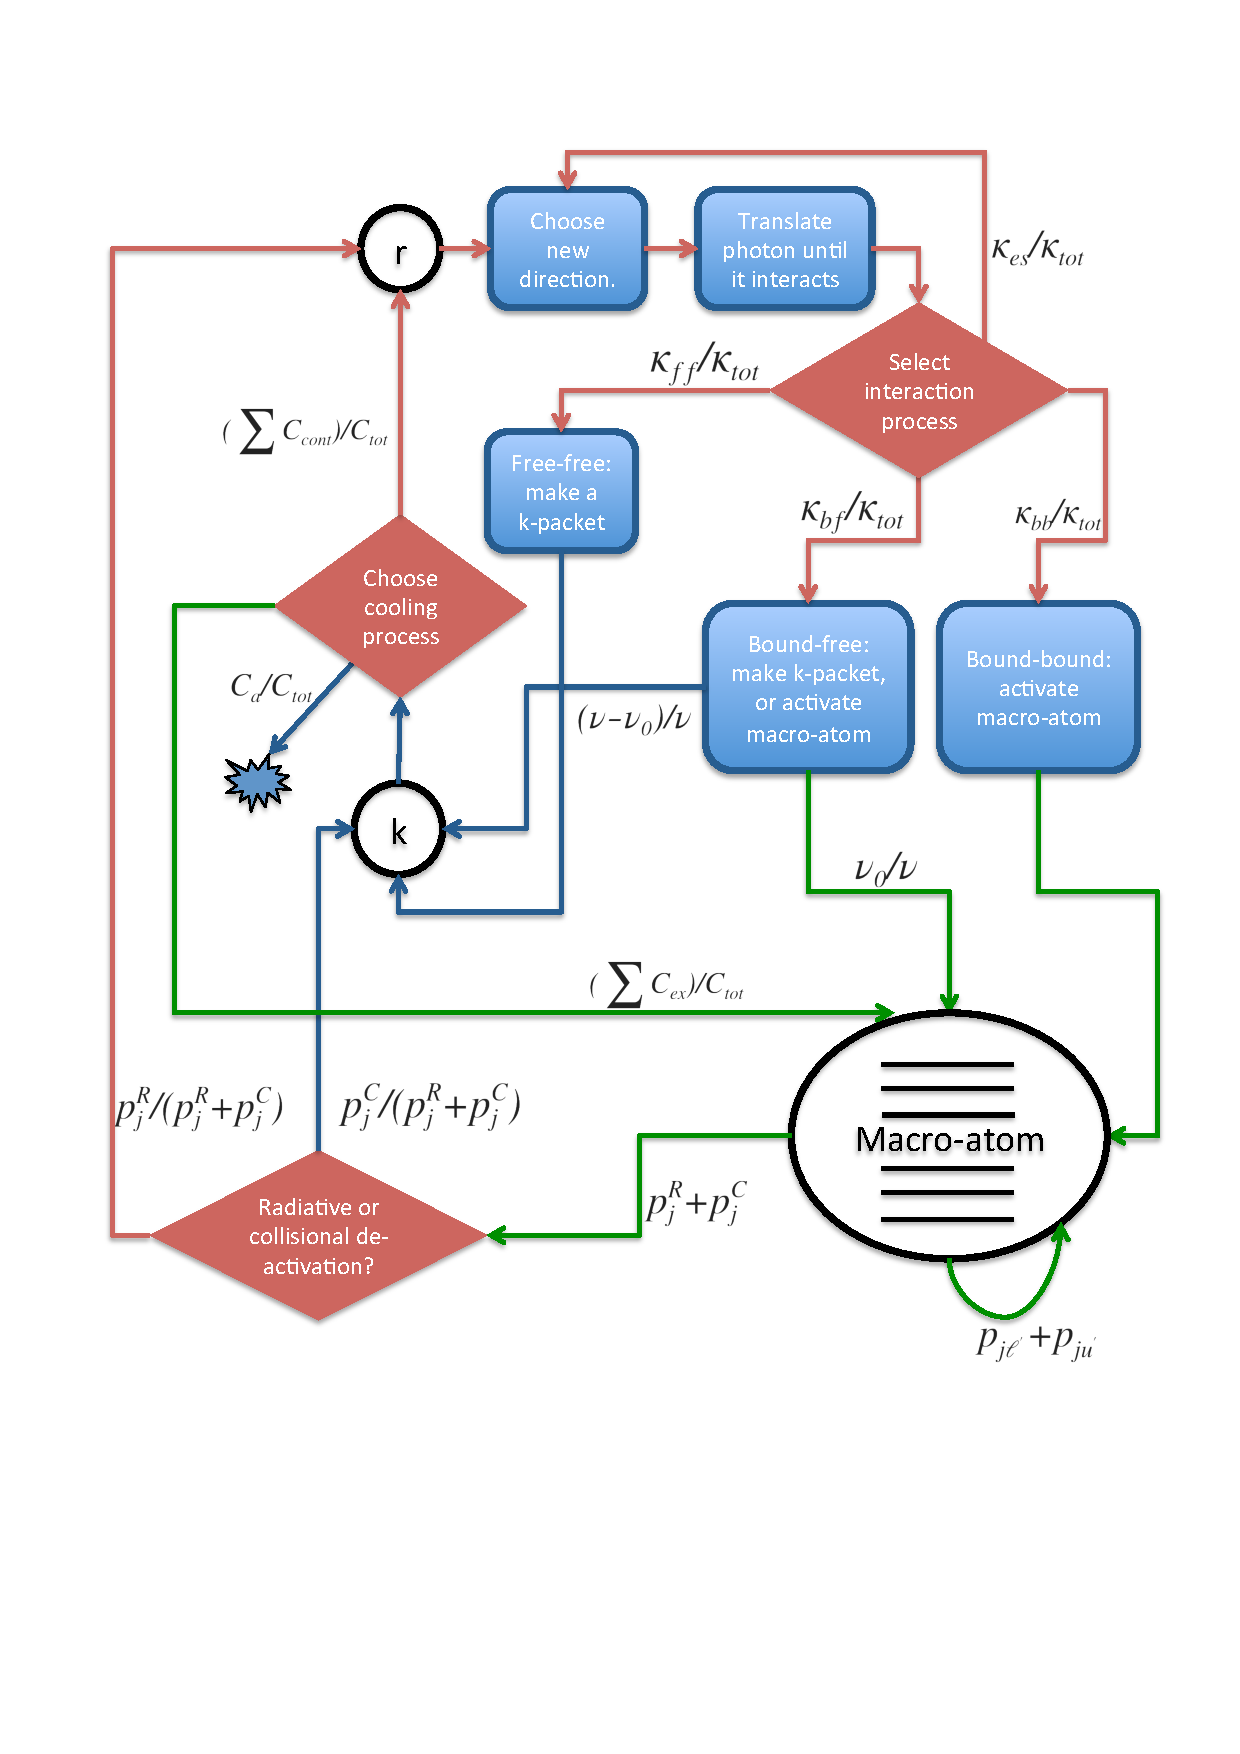
\includegraphics[width=1.0\textwidth, clip=true, trim=0 2.6in 0in 0in ]{figures/03-radtrans/matom_flow_ca.pdf}
\caption
[The decision tree traversed by an energy packet 
in macro-atom mode.]
{
The decision tree traversed by an energy packet 
in macro-atom mode, depicting the interaction
between radiation ($r$-packets), the thermal pool ($k$-packets), and ionization
and ionization/excitation energy (macro-atoms). 
The probabilities at each decision point are 
marked, and are defined in the text. The red, blue and green coloured arrows
represent radiant, kinetic and ionization/excitation energy respectively.
The symbols are defined in the text, except ${\cal C}_{\mathrm{cont}}$ and 
${\cal C}_{\mathrm{ex}}$ which refer to cooling contributions to radiative and excitation 
energy respectively.
} 
\label{fig:flow_matom}
\end{figure}

%% XXX CHECK THIS.


%%%%%%%%%%%%%%%%%%%%%%%%%%%%%
% POPS
%%%%%%%%%%%%%%%%%%%%%%%%%%%%%


\subsection{Ionization Fractions and Level Populations}
\label{sec:matom_pops}
In section~\ref{sec:lte} I described how it is possible to calculate the
ionization and excitation of a plasma under LTE or dilute approximations.
Macro-atoms are not approximated -- their level and ion populations are 
calculated by solving the rate equations formulated in section~\ref{sec:rate_eq}. 
This is done via matrix inversion. For an element with $n$ ions and $m_i$
levels in each ion, we construct a square matrix with dimensions 
$m = \sum_i^n m_i$.
This element then has a total number density of $N_{elem} = \sum_i^n N_i$.
To turn the system of rate equations for this element into matrix form, we
populate the $j$th diagonal of the matrix with the negative of the rate out of
level $j$, $-({\cal R}_{j\ellp} + {\cal R}_{j\up})$, 
and populate the off-diagonals $(j,k)$ with the positive rate 
${\cal R}_{jk}$. These are then multiplied by a vector of the fractional level
populations, and must equal a vector of zeros, due to statistical equilibrium.
Our matrix equation is then
%
\begin{equation}
\begin{bmatrix}
    -{\cal R}_{1\up} & {\cal R}_{21} & {\cal R}_{31} & \dots & {\cal R}_{m1} \\
    {\cal R}_{12} & -({\cal R}_{2\ellp} + {\cal R}_{2\up}) & {\cal R}_{32} & \dots & {\cal R}_{m2} \\
    {\cal R}_{13}  & {\cal R}_{23} & -({\cal R}_{3\ellp} + {\cal R}_{3\up}) & \dots & {\cal R}_{m3} \\
    \vdots & \vdots & \vdots & \ddots & \vdots \\
    {\cal R}_{1m}      & {\cal R}_{2m} & {\cal R}_{3m} & \dots & -{\cal R}_{m\ellp}
\end{bmatrix}
\begin{bmatrix}
    n_1 / N_{elem} \\
    n_2 / N_{elem} \\
    n_3 / N_{elem} \\
    \vdots         \\
    n_m / N_{elem} 
\end{bmatrix}
=
\begin{bmatrix}
    0 \\
    0 \\
    0 \\
    \vdots \\
    0
\end{bmatrix}
.
\end{equation}
%
This problem is not yet soluble, as a valid solution is that all levels 
could simply have occupation numbers of $0$. To close the problem, we must impose the boundary condition, that the sum of the fractional populations is 1, i.e.
%
\begin{equation}
\sum_i \frac{N_i}{N_{elem}} = 1.
\end{equation}
In matrix form, this is equivalent to replacing the entire first row
of the rate matrix with 1, and the first entry of the RHS vector with a 1,
so that we have
%
\begin{equation}
\begin{bmatrix}
    1  & 1 & 1 & \dots & 1\\
    {\cal R}_{12} & -({\cal R}_{2\ellp} + {\cal R}_{2\up}) & {\cal R}_{32} & \dots & {\cal R}_{m2} \\
    {\cal R}_{13}  & {\cal R}_{23} & -({\cal R}_{3\ellp} + {\cal R}_{3\up}) & \dots & {\cal R}_{m3} \\
    \vdots & \vdots & \vdots & \ddots & \vdots \\
    {\cal R}_{1m}      & {\cal R}_{2m} & {\cal R}_{3m} & \dots & -{\cal R}_{m\ellp}
\end{bmatrix}
\begin{bmatrix}
    n_1 / N_{elem} \\
    n_2 / N_{elem} \\
    n_3 / N_{elem} \\
    \vdots         \\
    n_m / N_{elem} 
\end{bmatrix}
=
\begin{bmatrix}
    1 \\
    0 \\
    0 \\
    \vdots \\
    0
\end{bmatrix}
\end{equation}
%
This matrix equation can now be solved.
To do the actual matrix manipulation, the code uses the GNU 
scientific libraries \citep[GSL;][]{GSL} implementation of
LU decomposition \citep{turing}. This is a fast and reliable way of
inverting large matrices that includes error handling and enables
checking of, for example, singular rate matrices.

\subsection{Numerical Issues and Population Inversions}
\label{sec:numerical_matom}

An inherent problem in MC simulations is noise, particularly
when the MC estimators involved rely on specific frequencies of
photons in order to be incremented. One of the side effects
of this is that population inversions can occur. A population
inversion is present when 
\begin{equation}
n_u > n_l \frac{g_u}{g_l}.
\label{eq:pop_inverse}
\end{equation}
This can cause clear problems, for example, with the inclusion
of the stimulated recombination rate as a negative photoionization
term. Inspection of equations~\ref{eq:einstein_relations} 
and \ref{eq:nlte_rul} reveals that a negative
excitation rate would be obtained in this situation.

To prevent this problem, the level populations are `cleaned' 
after calculation, as suggested by L03. 
This is done by cycling through the levels
after the above calculation has been carried our and checking if
condition~\ref{eq:pop_inverse} is ever satisfied. If it is, then
the upper population is simply set to a value just below this limit.
This is only necessary when there is a permitted dipole transition 
between the two levels being compared.

In addition to the population inversion problem, it is also possible to 
produce singular rate matrixes when photon statistics are poor, 
particularly in heavily absorbed portions of the wind where photons
which come into resonance with lines, or are above threshold frequencies,
may be rare. To deal with this issue, I have written a routine in \py\
that checks if the rate matrix is singular and if any anomalous (negative or
non-finite) populations exist in the solution found. If either of these 
conditions are met, then the calculation is redone using dilute estimators.
This procedure is also carried out for the simple-atom ionization
calculation when the rate matrix approach is in use 
(see section~\ref{sec:simple_ionization}).